\chapter{Future Work}
As mentioned in Conclusion Chapter, in the future, the whole workflow can be completed according to the current  techniques used in this project. It will enable YuMi to complete more holes up to finishing the entire shoe. In this chapter, several alternative methods to address the shoelace manipulation problem are discussed. 


\section{Gripper or External Wrist Camera} \label{futurecamera}

\begin{figure}[H]
\centering
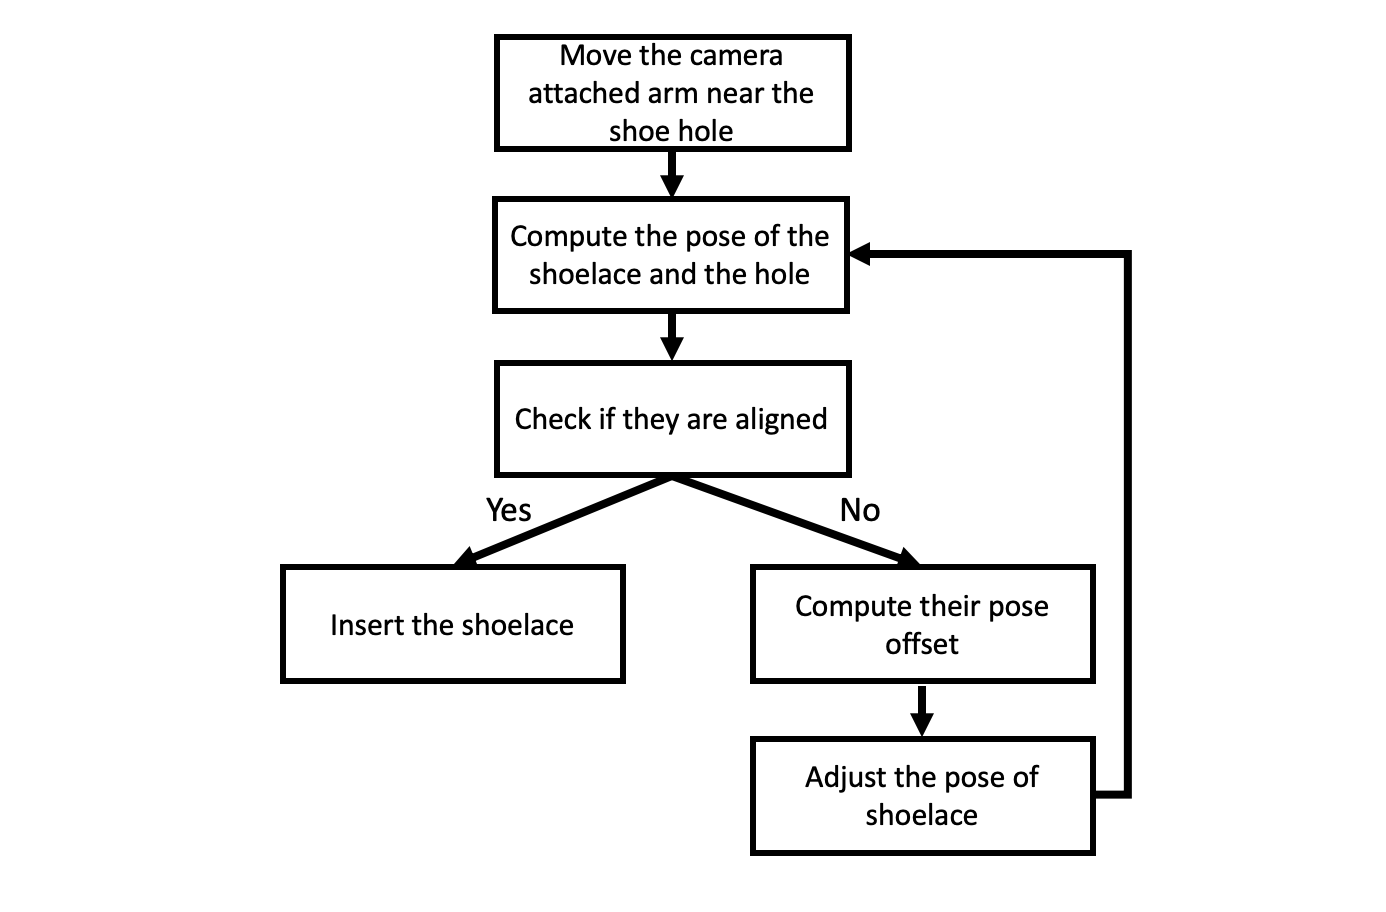
\includegraphics[width = 0.8\columnwidth]{Futurework/feedbackcamera.png}
\caption{Shoelace insertion workflow when using gripper or external wrist camera}
\label{feedbackcamera}
\end{figure}
Due to the reason that gripper camera of YuMi is currently unavailable, and attaching another small camera on YuMi's arm will limit YuMi's motion, this project only used one workspace camera eventually. When the gripper cameras become available or a suitable attaching way for wrist camera is found in the future, a more robust computer vision algorithm can be implemented, as shown in Figure \ref{feedbackcamera}.

For this approach, the wrist camera will detect and calculate the pose of shoe hole and shoelace, and only perform insertion if they are aligned. Ideally, this will improved the success rate of insertion task to 100\%. However, due to the additional computation and alignment, the execution time is considered to increase, which is the main drawback. 

\section{Shoe Model Construction}
As mentioned in Section \ref{oriestimation} of Background Chapter, there are numbers of existing methods to estimate the 6D pose of objects. By building shoe dataset that contains the photos and labels, and then retaining these models, the 6D pose of shoe can be computed in real-time. 

After that, the model of manipulated shoe need be constructed, which should contain the relative pose between every shoe hole and the centroid of the shoe. By doing this, once the pose estimation model gives the 6D pose of the shoe, every hole's pose can be determined accordingly. The motion planning algorithms can be applied directly afterwards. This approach is a combination of shoe detection, 3D location estimation and 3D orientation estimation discussed in this report. It is also not restricted by the color of shoes. 

However, this approach has one major drawback for shoes with soft uppers, because they are easily deformed. The shoe model needs to be reconstructed every time the shoe changes shape. Since building the model requires precise measurements and is time-consuming, this method is not applicable in this case.

\section{Deformable Object Tracking}
For regular shoelace without distinct color, color detection can not be applied. According to \citep{deformable_track}, the shoelace tracking problem can be addressed by using a probabilistic generative model that incorporates physical properties of tracked objects and its environments, as well as the point cloud sensor readings. 

\section{Reinforcement Learning}
This project can be extended to the area of reinforcement learning (RL), which enables the autonomous robot to learn behavioral skills directly from experience and interaction in the real world. RL can process complex sensory input using general purpose neural network (NN) and pick the action to maximize the cumulative reward. The basic RL system is characterized by actor and critic modules. To be specific, the actor interacts with the shoe or shoe hole by selecting system actions given a specific input state. While the critic provides the feedback about how successful the actions were (such as how close to the shoelace and shoe hole were etc), which is used to refine the action.

However, many existing RL algorithms need weeks of real-world data to converge to the desired behavior. In addition, this can be difficult to deploy on complex robotic systems. \citep{reinforcementl} demonstrated a deep RL based on off-policy training of deep Q functions can learn NN policies efficiently, and train on the real physical robot to perform complex 3D manipulation tasks such as door opening. \citep{drlsac} presented Soft-Actor-Critic, a off-policy actor-critic algorithm based on the maximum entropy RL framework. It was also be evaluated on several benchmark tasks including robotic manipulation with a dexterous hand.


%However, there is a trade-off between the autonomy of the learning process and the training time. Human supplied demonstration and hand engineered policy are typically involved. This limitation can be alleviated by deep RL which trains general-purpose neural network (NN) policies, but the applications are restricted to simple tasks due to their high sample complexity. 